\documentclass[a4paper,12pt,onecolumn]{article}

\usepackage[english]{babel}
\usepackage{amssymb,amsmath,array,epsfig,a4,subfig}


\newcommand{\errorXx}{\|\Gamma^h - \Gamma\|_{L^\infty}}
\newcommand{\LerrorUu}[1]{\|\vec U - I^h_{#1}\,\vec u\|_{L^2(\Omega_T)}}
\newcommand{\errorUu}[1]{\|\vec U - I^h_{#1}\,\vec u\|_{L^\infty}}
\newcommand{\errorPp}[1]{\|P - I^h_{#1}\,p\|_{L^\infty}}
\newcommand{\LerrorPp}{\|P - p\|_{L^2(\Omega_T)}}

\begin{document}

\captionsetup[subfigure]{labelformat=empty} % remove label subplot
\newcolumntype{H}{>{\setbox0=\hbox\bgroup}c<{\egroup}@{}} % hide table column

\section{Miscellaneous}

\begin{figure}[htbp]
\centering
\includegraphics[width=.45\textwidth]
{figures/2d_stationary_bubble_adaptive_100.ps}
\caption{($\mu=\gamma=1$) Pressure of the 2d stationary bubble at time $t=1$
for the P2--P0 element.}
\end{figure}

\begin{figure}[htbp]
  \centering
  \subfloat[$t=0$]{\includegraphics[width=.45\textwidth]
  {figures/expanding_bubble_uniform_000.ps}}\\
  \subfloat[$t=0.25$]{\includegraphics[width=.45\textwidth]
  {figures/expanding_bubble_uniform_025.ps}}
  \subfloat[$t=0.5$]{\includegraphics[width=.45\textwidth]
  {figures/expanding_bubble_uniform_050.ps}}\\
  \subfloat[$t=0.75$]{\includegraphics[width=.45\textwidth]
  {figures/expanding_bubble_uniform_075.ps}}
  \subfloat[$t=1$]{\includegraphics[width=.45\textwidth]
  {figures/expanding_bubble_uniform_100.ps}}
\caption{($\mu_+ = 10\,\mu_- = \gamma = 1,\alpha = 0.15$) Pressure evolution of
the 2d expanding bubble for the P2--P0 element, $C_r=3$.}
\end{figure}

In order to choose the better remeshing coefficient $C_r$ several experiment
were carried out. Some errors for our approximation are shown in
Table~\ref{tab:expandingbubble2Dp2p0bothdiffcr} with a starting characteristic
length $c_l=0.1$, using P2--P0 polynomials and smoothing coefficient $C_s=1$.
The better result are obtained with $C_r=3$ because it reduces the number of
remeshing compared to $C_r=2$ while keeping the same performance and error
quality. For this reason we are going to use this parameter for the other
simulations.
\begin{table*}
 \center
\begin{tabular}{llHllHll}
\hline
$C_r$ & $\errorXx$ & $\LerrorUu2$ & $\errorUu2$ & $\LerrorPp$ & $\errorPp0$ &
$CPU[s]$ & $K_\Omega^T$\\
\hline
2 & 1.46658e-03 & 1.05801e-04 & 8.73227e-04 & 2.14589e-01 & 3.68834e-02 & 4297
& 452\\
3 & 1.47162e-03 & 1.02085e-04 & 7.19650e-04 & 2.13599e-01 & 3.68834e-02 & 3919
& 468\\
4 & 1.46761e-03 & 1.27330e-04 & 8.55458e-04 & 2.19071e-01 & 3.68834e-02 & 4682
& 504\\
5 & 1.47218e-03 & 1.26419e-04 & 7.20711e-04 & 2.12456e-01 & 3.68834e-02 & 4775&
468\\
\hline
\end{tabular}
\caption{($\mu_+ = 10\,\mu_- = \gamma = 1,\alpha = 0.15$) Expanding bubble
problem on $(-1,1)^2\setminus[-\frac{1}{3},\frac{1}{3}]^2$ over the time
interval $[0,1]$ for the P2--P0 element, $C_s=1$, $c_l=0.1$ and uniform mesh.}
\label{tab:expandingbubble2Dp2p0bothdiffcr}
\end{table*}

In all the previous simulations, the meshes used were uniform therefore the
characteristic length was equal for all the nodes. Moreover they were kept
uniform also after the remeshing. Obviously, with this approach, it is very
expensive to have a large number of interface elements since it leads to a
drastic increase of bulk elements. In the following simulations, instead, we use
adaptive meshes which are fine close to the interface and coarse far from the
interface.

Instead, in Figure~\ref{fig:shear_2d_smooth} the remeshing coefficient is
$C_r=0$ so only the smoothing is used. The bulk inner relative volume evolution
is reported in Figure~\ref{fig:shear_2d_smooth_bulk_inner_volume}.
\begin{figure}[htbp]
  \centering
  \subfloat[$t=0.5$]{\includegraphics[width=.45\textwidth]
  {figures/2d_shear_smooth_050.ps}}\quad
  \subfloat[$t=1$]{\includegraphics[width=.45\textwidth]
  {figures/2d_shear_smooth_100.ps}}\\
  \subfloat[$t=2.5$]{\includegraphics[width=.45\textwidth]
  {figures/2d_shear_smooth_250.ps}}\quad
  \subfloat[$t=5$]{\includegraphics[width=.45\textwidth]
  {figures/2d_shear_smooth_500.ps}}\\
  \caption{($\mu=1,\gamma=3$) Pressure evolution of the 2D shear flow with
$c_l=0.05$, $C_s=1$ and no remeshing for the P2--P0 element, uniform mesh.}
  \label{fig:shear_2d_smooth}
\end{figure}

\begin{figure}[htbp]
  \centering
  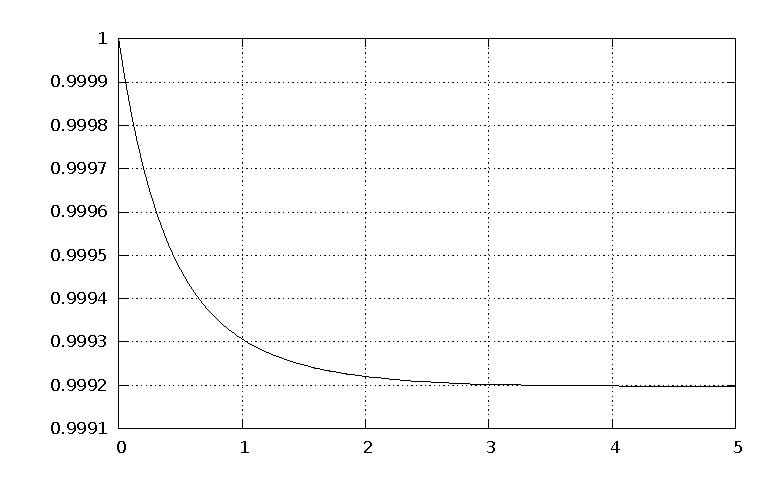
\includegraphics[width=.45\textwidth]
  {figures/2d_shear_smooth_bulk_inner_volume.ps}
  \caption{($\mu=\gamma=1$) Bulk inner relative volume evolution of the 2D
shear flow with $c_l=0.05$, $C_s=1$ and no remeshing for the P2--P0 element,
uniform mesh.}
  \label{fig:shear_2d_smooth_bulk_inner_volume}
\end{figure}

TODO : add comparison reults unfitted scheme scheme stokes paper

The P2--P0 element has the same accuracy of the P2--(P1+P0) element but it is
simpler to implement, always satisfies the LBB condition and the resulting
linear system is smaller therefore it is the best choice.

The adaptive mesh works very well for the stationary bubble problem. Indeed,
with a fraction of bulk elements, it reaches the same accuracy of the uniform
mesh. Unfortunately this is not the case for the expanding bubble problem. For
this problem, the uniform mesh is much faster and requires less bulk elements
compared to the adaptive mesh therefore.\footnote{But they have different
$\tau$!}

In the 2D expanding bubble problem, We can observe that the simulations which
use only the smoothing have bigger errors and take more time therefore it is not
feasible to use only the smoothing process. On the other side both only
remeshing and smoothing/remeshing combined achieve almost the same quality and
performance. It is important to notice that the performance are almost the same
for sequential code (our case) but in parallel computation the remeshing is the
real bottleneck therefore it is way better to use the combined
smoothing/remeshing approach.

Both element capture perfectly the jump in the pressure.
\end{document}
